\chapter{Results and Discussion}
\label{ch:results}

\section{Overall Out-of-Sample Performance}
Out-of-sample evaluation was conducted across four chronological 2-year test segments spanning 2018 through 2025. Table~\ref{tab:overall_results} presents the pooled test performance metrics (averaged across four folds and three random seeds) for models M1--M4 alongside the passive Equal-Weight (EW) 1/N benchmark.

\begin{table}[htbp]
\centering
\footnotesize
\setlength{\tabcolsep}{3pt}
\caption{Pooled out-of-sample test performance across 4 folds and 3 seeds (mean $\pm$ standard deviation).}
\label{tab:overall_results}
\begin{tabular}{lcccccc}
\toprule
\textbf{Model} & \textbf{Cum. Return (\%)} & \textbf{CAGR (\%)} & \textbf{Sharpe Ratio} & \textbf{Sortino} & \textbf{Max DD (\%)} & \textbf{Cost (\% of $V_0$)} \\
\midrule
\textbf{M1 (MLP)} & $20.62 \pm 5.14$ & $9.90 \pm 2.31$ & $0.71 \pm 0.13$ & $1.03 \pm 0.20$ & $-19.50 \pm 1.04$ & $9.68 \pm 0.10$ \\
\textbf{M2 (LSTM)} & $28.23 \pm 2.03$ & $13.37 \pm 0.88$ & $0.92 \pm 0.07$ & $1.34 \pm 0.09$ & $-18.52 \pm 1.35$ & $4.27 \pm 1.44$ \\
\textbf{M3 (+ DSR)} & $26.93 \pm 3.27$ & $12.68 \pm 1.56$ & $0.92 \pm 0.11$ & $1.34 \pm 0.17$ & $-19.95 \pm 0.81$ & $4.14 \pm 1.15$ \\
\textbf{M4 (+ Turn. Pen.)} & $20.97 \pm 4.19$ & $10.09 \pm 1.85$ & $0.92 \pm 0.17$ & $1.37 \pm 0.26$ & $\mathbf{-16.04 \pm 1.72}$ & $\mathbf{0.97 \pm 0.15}$ \\
\midrule
\textbf{Equal-Weight} & $\mathbf{36.48}$ & $\mathbf{17.08}$ & $\mathbf{1.13}$ & $\mathbf{1.66}$ & $-18.91$ & $\mathbf{0.61}$ \\
\bottomrule
\end{tabular}
\end{table}

Figure~\ref{fig:equity_stitched} illustrates cumulative out-of-sample portfolio profit (assuming $V_0 = \text{INR } 1{,}000{,}000$ initial capital reinvested sequentially) across the continuous 2018--2025 timeline. Figure~\ref{fig:drawdown} portrays peak-to-trough drawdowns, and Figure~\ref{fig:profit_bars} depicts profit across each 2-year test window.

\begin{figure}[htbp]
\centering
\begin{minipage}{0.49\textwidth}
\centering
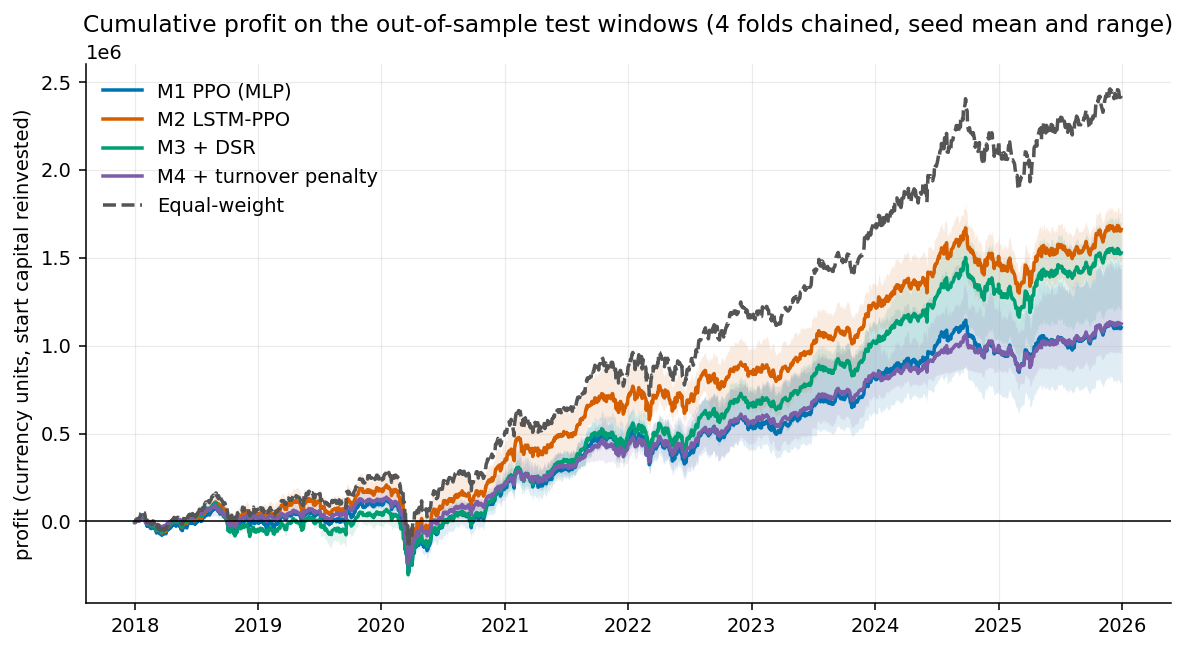
\includegraphics[width=\textwidth]{equity_stitched.png}
\caption{Cumulative out-of-sample profit across 4 chained test windows (2018--2025).}
\label{fig:equity_stitched}
\end{minipage}\hfill
\begin{minipage}{0.49\textwidth}
\centering
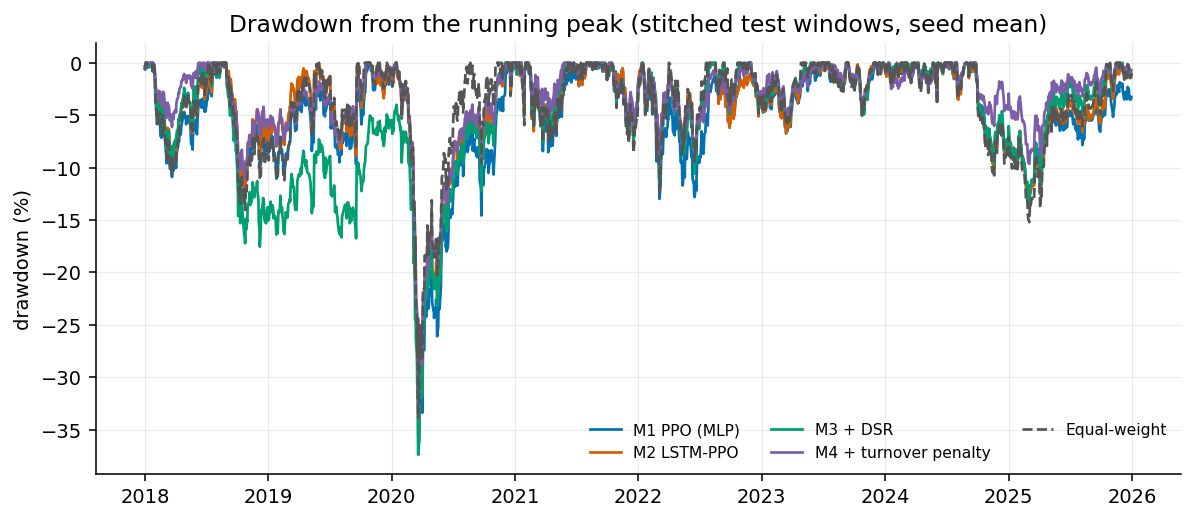
\includegraphics[width=\textwidth]{drawdown.png}
\caption{Out-of-sample portfolio drawdown from running peak (2018--2025).}
\label{fig:drawdown}
\end{minipage}
\end{figure}

\section{Analysis of Ablation Steps}
To establish statistical significance, paired difference tests were computed across all (fold, seed) tuples using 10,000-sample fold-level bootstrap resampling. Table~\ref{tab:ablation_deltas} reports the resulting paired deltas and 95\% confidence intervals.

\begin{table}[htbp]
\centering
\scriptsize
\setlength{\tabcolsep}{2.5pt}
\caption{Paired ablation differences ($b - a$) with 95\% bootstrap confidence intervals.}
\label{tab:ablation_deltas}
\begin{tabular}{llcccc}
\toprule
\textbf{Ablation Transition} & \textbf{Metric} & \textbf{Mean Delta} & \textbf{95\% CI} & \textbf{Folds Improved} & \textbf{Pairs Improved} \\
\midrule
\multirow{4}{*}{\textbf{M1 $\to$ M2} (Temporal Memory)} 
& Sharpe Ratio & $+0.201$ & $[+0.156, +0.246]$ & $4 / 4$ & $9 / 12$ \\
& Cum. Return (\%) & $+7.61\%$ & $[+4.81\%, +10.01\%]$ & $4 / 4$ & $10 / 12$ \\
& Daily Turnover & $-0.106$ & $[-0.138, -0.070]$ & $4 / 4$ & $11 / 12$ \\
& Cost (\% of $V_0$) & $-5.41\%$ & $[-7.37\%, -3.34\%]$ & $4 / 4$ & $11 / 12$ \\
\midrule
\multirow{4}{*}{\textbf{M2 $\to$ M3} (DSR Reward)} 
& Sharpe Ratio & $+0.003$ & $[-0.295, +0.222]$ & $3 / 4$ & $7 / 12$ \\
& Cum. Return (\%) & $-1.30\%$ & $[-9.33\%, +4.45\%]$ & $2 / 4$ & $6 / 12$ \\
& Max Drawdown (\%) & $-1.43\%$ & $[-5.36\%, +0.81\%]$ & $3 / 4$ & $6 / 12$ \\
& Daily Turnover & $-0.002$ & $[-0.019, +0.014]$ & $2 / 4$ & $7 / 12$ \\
\midrule
\multirow{4}{*}{\textbf{M3 $\to$ M4} (Turnover Penalty)} 
& Sharpe Ratio & $+0.005$ & $[-0.236, +0.280]$ & $2 / 4$ & $6 / 12$ \\
& Cum. Return (\%) & $-5.96\%$ & $[-13.29\%, +3.37\%]$ & $1 / 4$ & $3 / 12$ \\
& Max Drawdown (\%) & $\mathbf{+3.90\%}$ & $[+1.45\%, +7.00\%]$ & $\mathbf{4 / 4}$ & $\mathbf{10 / 12}$ \\
& Daily Turnover & $\mathbf{-0.060}$ & $[-0.082, -0.044]$ & $\mathbf{4 / 4}$ & $\mathbf{12 / 12}$ \\
& Cost (\% of $V_0$) & $\mathbf{-3.17\%}$ & $[-4.01\%, -2.43\%]$ & $\mathbf{4 / 4}$ & $\mathbf{12 / 12}$ \\
\midrule
\multirow{4}{*}{\textbf{M1 $\to$ M4} (All Combined)} 
& Sharpe Ratio & $+0.209$ & $[+0.012, +0.386]$ & $3 / 4$ & $8 / 12$ \\
& Max Drawdown (\%) & $+3.45\%$ & $[+2.52\%, +4.03\%]$ & $4 / 4$ & $8 / 12$ \\
& Daily Turnover & $-0.167$ & $[-0.190, -0.144]$ & $4 / 4$ & $12 / 12$ \\
& Cost (\% of $V_0$) & $-8.71\%$ & $[-10.07\%, -7.27\%]$ & $4 / 4$ & $12 / 12$ \\
\bottomrule
\end{tabular}
\end{table}

\subsection{Step 1: Impact of Temporal Memory (M2 versus M1)}
Transitioning from the MLP (M1) to the LSTM (M2) constitutes the single most consequential enhancement in the ablation hierarchy. The Sharpe ratio rises significantly from $0.714$ to $0.915$ ($+0.201$, 95\% CI $[+0.156, +0.246]$), improving across all four folds ($4/4$). Simultaneously, daily turnover plummets by more than half, from $0.186$ to $0.080$, reducing total transaction costs from $9.68\%$ to $4.27\%$ of starting capital. 

The MLP observes only the current day's normalized state, causing it to react erratically to day-to-day market noise. In contrast, the internal memory cells of the LSTM smooth out short-term oscillations and track persistent medium-term trends, generating substantial execution savings.

\subsection{Step 2: Impact of Differential Sharpe Ratio (M3 versus M2)}
Replacing raw net return with the Differential Sharpe Ratio (M3) yields an incremental Sharpe delta of $+0.003$ ($[-0.295, +0.222]$). While M3 maintains high Sharpe ratios in Folds 3 and 4 ($1.328$ and $1.164$), its out-of-sample return is slightly lower than M2 ($26.93\%$ vs.\ $28.23\%$). The recursive exponential moving average of DSR dampens aggressive rebalancing during trending bull markets, curtailing profit capture while modestly stabilising risk metrics.

\subsection{Step 3: Impact of Turnover Regularisation (M4 versus M3)}
Incorporating the quadratic turnover penalty in Model M4 produces a decisive shift in trading behaviour:
\begin{itemize}
    \item \textbf{Drastic Cost Reduction:} Average daily turnover drops from $0.079$ to $0.019$ (a 76\% reduction), bringing total transaction costs down to $0.97\%$ of starting capital, which closely approaches the passive benchmark ($0.61\%$).
    \item \textbf{Superior Downside Protection:} Max drawdown improves by $+3.90\%$ (from $-19.95\%$ to $-16.04\%$, 95\% CI $[+1.45\%, +7.00\%]$), achieving the shallowest drawdown among all models, including Equal-Weight ($-18.91\%$).
    \item \textbf{Trading Frictions and Turnover:} Figure~\ref{fig:turnover_cost} explicitly demonstrates the collapse in trading activity and transaction friction across the ablation sequence.
\end{itemize}

\begin{figure}[htbp]
\centering
\begin{minipage}{0.49\textwidth}
\centering
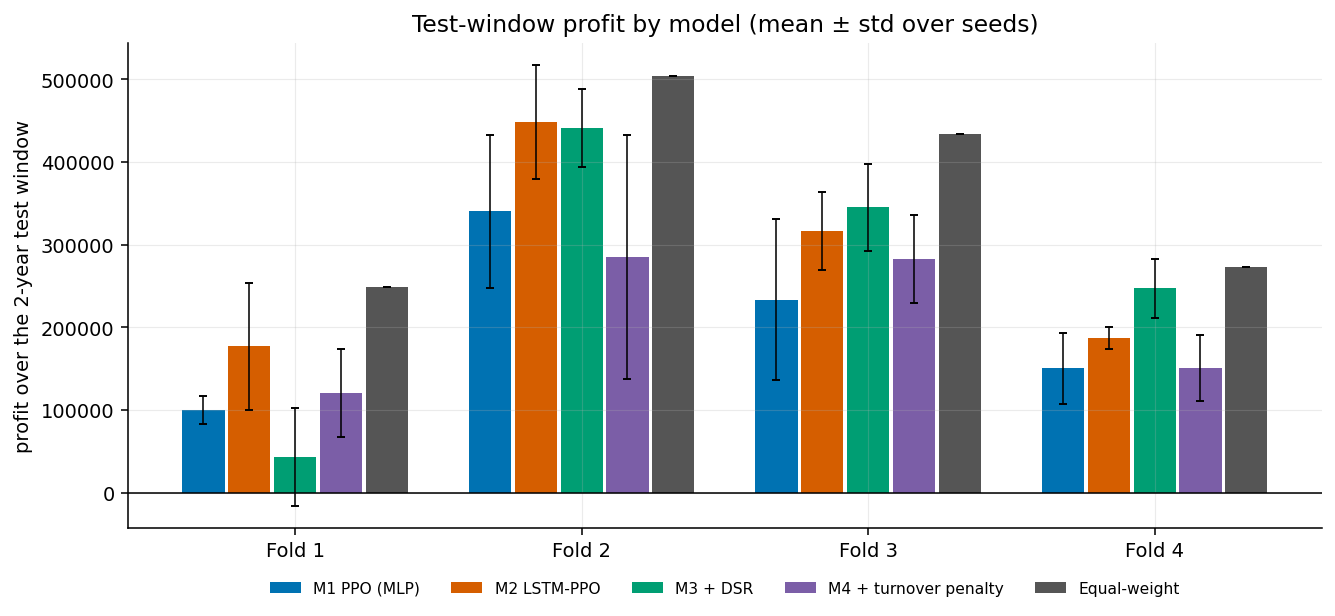
\includegraphics[width=\textwidth]{profit_bars.png}
\caption{Profit per 2-year test window by model.}
\label{fig:profit_bars}
\end{minipage}\hfill
\begin{minipage}{0.49\textwidth}
\centering
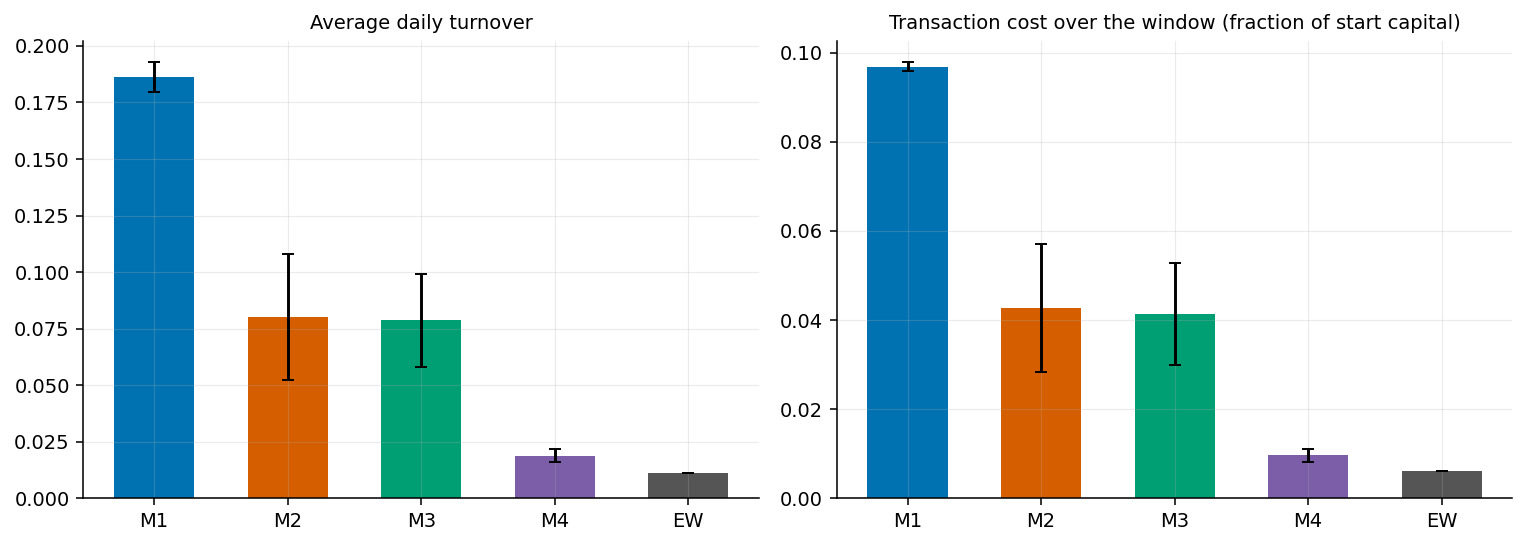
\includegraphics[width=\textwidth]{turnover_cost.png}
\caption{Average daily turnover and transaction costs.}
\label{fig:turnover_cost}
\end{minipage}
\end{figure}

\section{Fold-by-Fold Performance Dynamics}
Table~\ref{tab:per_fold_results} provides the breakdown of cumulative returns across each fold. Performance exhibits marked regime dependence:
\begin{itemize}
    \item \textbf{Fold 1 (2018--2019):} Moderate growth environment. All RL models generate positive return ($10.0\%$ to $17.8\%$), though trailing EW ($24.9\%$).
    \item \textbf{Fold 2 (2020--2021):} Highly volatile pandemic crash and subsequent massive recovery. M2 and M3 capture dramatic gains ($44.8\%$ and $44.1\%$), whereas M4 lagged ($28.5\%$) because its turnover penalty discouraged rapid capital reallocation during the rapid post-crash rebound.
    \item \textbf{Fold 3 (2022--2023):} Inflationary cycle and sector rotation. M3 achieves its strongest risk-adjusted performance with a Sharpe ratio of $1.328$, closely tracking EW ($34.5\%$ vs.\ $43.4\%$).
    \item \textbf{Fold 4 (2024--2025):} Secular bull market. M3 delivers $24.7\%$ return, outperforming M1 and M4.
\end{itemize}

\begin{table}[htbp]
\centering
\small
\caption{Out-of-sample cumulative return (\%) per walk-forward fold (mean $\pm$ standard deviation over seeds).}
\label{tab:per_fold_results}
\begin{tabular}{lccccc}
\toprule
\textbf{Fold Window} & \textbf{Model M1} & \textbf{Model M2} & \textbf{Model M3} & \textbf{Model M4} & \textbf{Equal-Weight} \\
\midrule
Fold 1 (2018--2019) & $10.0 \pm 1.7$ & $17.8 \pm 7.7$ & $4.4 \pm 5.9$ & $12.1 \pm 5.3$ & $\mathbf{24.9}$ \\
Fold 2 (2020--2021) & $34.0 \pm 9.2$ & $44.8 \pm 6.9$ & $44.1 \pm 4.7$ & $28.5 \pm 14.8$ & $\mathbf{50.4}$ \\
Fold 3 (2022--2023) & $23.4 \pm 9.7$ & $31.6 \pm 4.7$ & $34.5 \pm 5.2$ & $28.3 \pm 5.3$ & $\mathbf{43.4}$ \\
Fold 4 (2024--2025) & $15.0 \pm 4.2$ & $18.7 \pm 1.3$ & $24.7 \pm 3.6$ & $15.1 \pm 4.0$ & $\mathbf{27.3}$ \\
\midrule
\textbf{Pooled Mean} & $20.6 \pm 5.1$ & $28.2 \pm 2.0$ & $26.9 \pm 3.3$ & $21.0 \pm 4.2$ & $\mathbf{36.5}$ \\
\bottomrule
\end{tabular}
\end{table}

\section{Equal-Weight Benchmark Outperformance and Gap Decomposition}
In the final experimental test, the passive Equal-Weight benchmark achieved the highest cumulative profit ($36.48\%$ pooled return, Sharpe 1.131), outperforming all four RL models. Rather than obscuring this finding, we perform a rigorous return gap decomposition to understand why active RL underperformed 1/N.

Table~\ref{tab:gap_decomp} decomposes the cumulative return shortfall into two orthogonal components:
\begin{enumerate}
    \item \textbf{Cash Drag:} The return forfeited by holding an uninvested cash allocation during an overall upward-trending market.
    \item \textbf{Stock Choice and Timing:} The differential return resulting from active equity weight deviations relative to equal-weighting across the ten equities.
\end{enumerate}

\begin{table}[htbp]
\centering
\footnotesize
\setlength{\tabcolsep}{4pt}
\caption{Decomposition of cumulative out-of-sample return gap against Equal-Weight (\% points).}
\label{tab:gap_decomp}
\begin{tabular}{lccccc}
\toprule
\textbf{Model} & \textbf{EW Return} & \textbf{Cash Drag} & \textbf{EW Same Cash} & \textbf{Stock Selection} & \textbf{Model Return} \\
\midrule
\textbf{M1 (MLP)} & $135.66$ & $-13.67$ & $121.99$ & $-2.11$ & $119.88$ \\
\textbf{M2 (LSTM)} & $135.66$ & $-9.99$ & $125.67$ & $-2.14$ & $123.53$ \\
\textbf{M3 (+ DSR)} & $135.66$ & $-15.14$ & $120.52$ & $-3.32$ & $117.20$ \\
\textbf{M4 (+ Turn. Pen.)} & $135.66$ & $\mathbf{-42.35}$ & $93.31$ & $-7.84$ & $\mathbf{85.47}$ \\
\bottomrule
\end{tabular}
\end{table}

Table~\ref{tab:avg_weights} reports the average portfolio allocations across the entire evaluation horizon. 

\begin{table}[htbp]
\centering
\scriptsize
\setlength{\tabcolsep}{2.5pt}
\caption{Average asset allocations across models over the out-of-sample evaluation period.}
\label{tab:avg_weights}
\begin{tabular}{lccccccccccc}
\toprule
\textbf{Model} & \textbf{RELI} & \textbf{TCS} & \textbf{HDFCB} & \textbf{ICICIB} & \textbf{ITC} & \textbf{HIND} & \textbf{LT} & \textbf{SUNP} & \textbf{MARU} & \textbf{BHAR} & \textbf{Cash} \\
\midrule
\textbf{M1} & 0.088 & 0.120 & 0.085 & 0.087 & 0.084 & 0.077 & 0.091 & 0.087 & 0.087 & 0.094 & \textbf{0.101} \\
\textbf{M2} & 0.098 & 0.144 & 0.073 & 0.091 & 0.081 & 0.087 & 0.082 & 0.090 & 0.098 & 0.071 & \textbf{0.087} \\
\textbf{M3} & 0.089 & 0.119 & 0.073 & 0.077 & 0.072 & 0.079 & 0.073 & 0.094 & 0.107 & 0.086 & \textbf{0.131} \\
\textbf{M4} & 0.066 & 0.103 & 0.079 & 0.061 & 0.049 & 0.066 & 0.057 & 0.071 & 0.092 & 0.032 & \textbf{0.324} \\
\textbf{EW} & 0.100 & 0.100 & 0.100 & 0.100 & 0.100 & 0.100 & 0.100 & 0.100 & 0.100 & 0.100 & \textbf{0.000} \\
\bottomrule
\end{tabular}
\end{table}

The empirical cause of benchmark outperformance is unequivocal:
\begin{itemize}
    \item Between 2018 and 2025, the Indian equity market experienced a sustained structural bull market. The passive 1/N benchmark remained 100\% invested across all ten large-cap stocks at all times, incurring minimal rebalancing friction ($0.61\%$).
    \item Model M4 learned to allocate an average of \textbf{32.4\%} of its portfolio to cash to minimize volatility and avoid turnover penalties. This cash buffer caused a massive $-42.35\%$ cash drag relative to Equal-Weight. In contrast, stock timing accounted for only $-7.84\%$ deficit.
    \item Thus, M4's lower return was not caused by poor stock picking, but by its risk-averse preference for capital preservation in cash during a high-momentum bull market.
\end{itemize}

\section{M4 Hyperparameter Tuning and Validation Dynamics}
Figure~\ref{fig:m4_sweep} depicts the hyperparameter sweep over $\lambda_{\text{turn}} \in \{0.01, 0.03, 0.1, 0.3\}$ on Fold 1 validation across two random seeds (seeds 0 and 1).

\begin{figure}[htbp]
\centering
\begin{minipage}{0.49\textwidth}
\centering
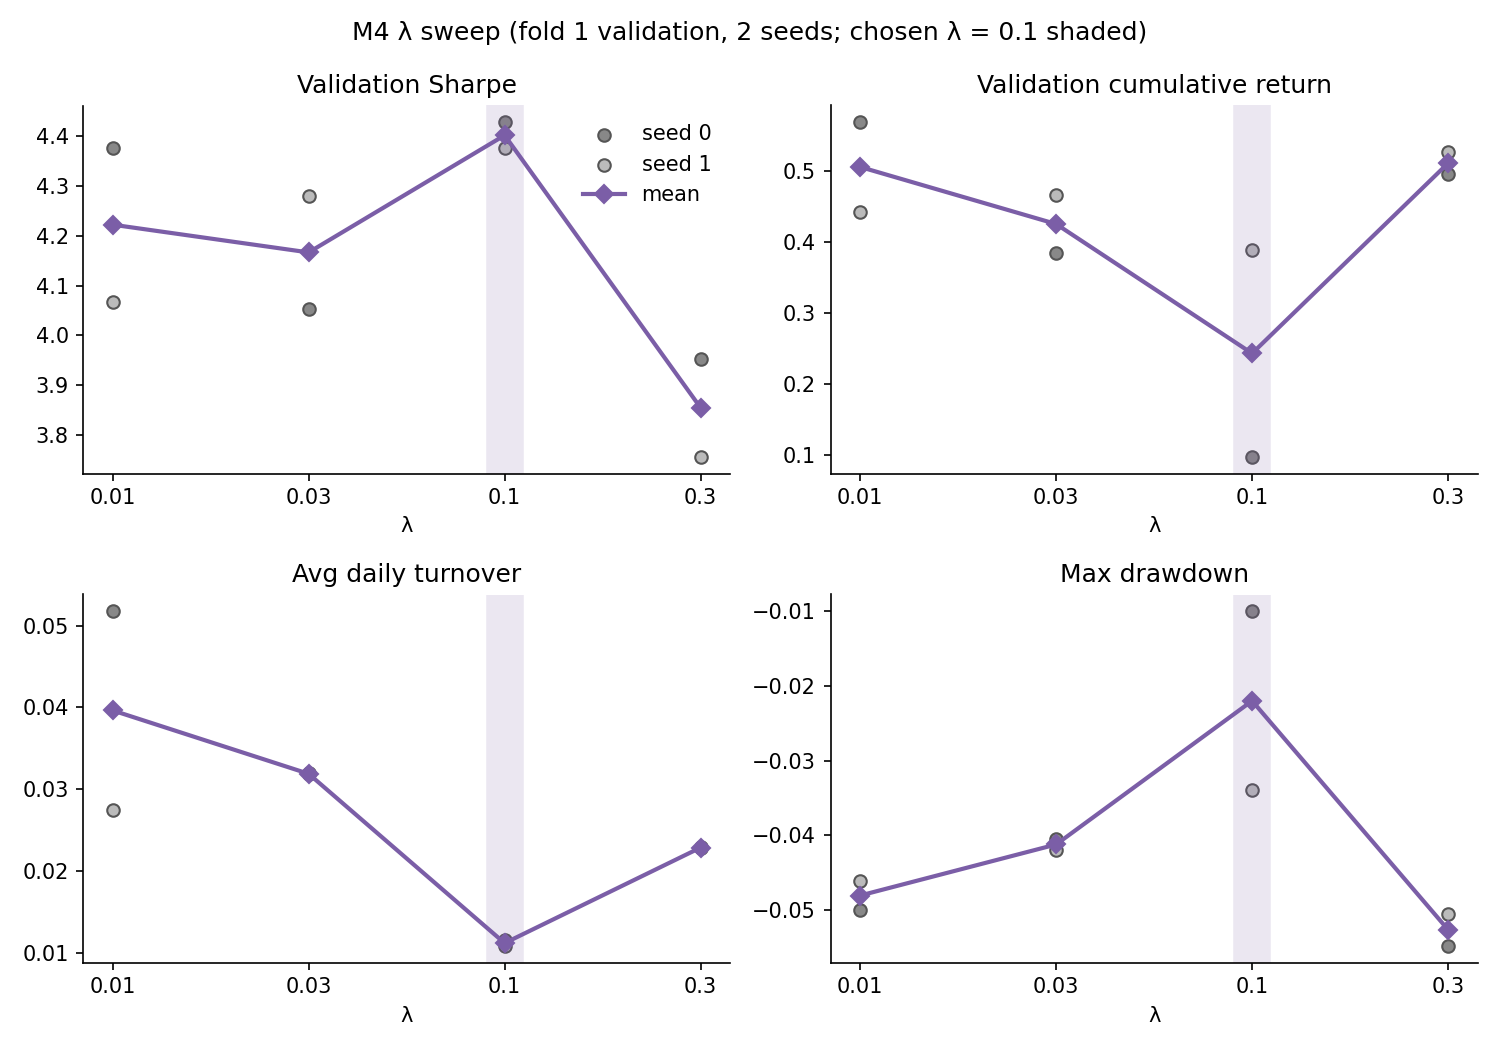
\includegraphics[width=\textwidth]{m4_lambda_sweep.png}
\caption{M4 turnover penalty parameter sweep (chosen $\lambda=0.1$ shaded).}
\label{fig:m4_sweep}
\end{minipage}\hfill
\begin{minipage}{0.49\textwidth}
\centering
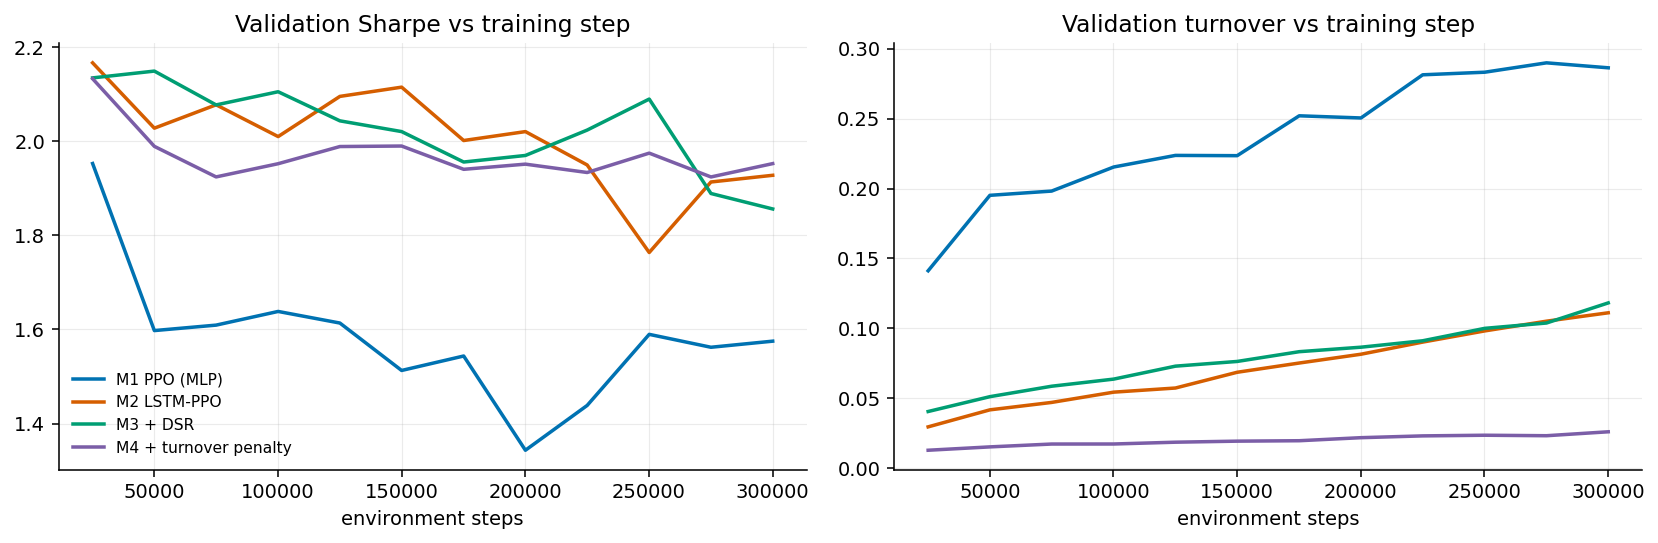
\includegraphics[width=\textwidth]{validation_curves.png}
\caption{Validation Sharpe and turnover dynamics over 300,000 steps.}
\label{fig:val_curves}
\end{minipage}
\end{figure}

The grid sweep demonstrates that $\lambda = 0.1$ achieved the optimal trade-off on Fold 1 validation, maximizing the mean validation Sharpe ratio ($4.40$) while curtailing validation drawdown to $-2.2\%$. At $\lambda = 0.01$, turnover remains high ($0.040$), whereas at $\lambda = 0.3$, the penalty stifles necessary reallocations. We explicitly note as a limitation that $\lambda_{\text{turn}} = 0.1$ was selected on Fold 1 alone across two seeds and applied frozen across all folds. Finally, the validation curves show clear over-training beyond 100,000 steps, highlighting the critical importance of checkpoint early stopping.
